\documentclass[aspectratio=169]{beamer}

\usepackage{listings}
\usetheme{ccc}

\lstset{language=Haskell, basicstyle=\small}


\author{Justus Adam}
\title{Why Data is the Better Monad}
\subtitle{Using Freedom to Great Effect}

\AtBeginSection[]
{
  \begin{frame}
    \frametitle{Table of Contents}
    \tableofcontents[currentsection]
  \end{frame}
}

\begin{document}

\frame{\titlepage}

\begin{frame}{Table of Contents}
  \tableofcontents
\end{frame}

\section{Recap: Monads}

\begin{frame}
  \frametitle{Why Monads?}
  \begin{itemize}
  \item Answer to the question ``How to do pure side effects?''
  \item Associates values with side effects used for its production
  \item Can be thought of as an environment for a value
  \item Most iconic Monad: \texttt{IO}
  \end{itemize}
\end{frame}

\begin{frame}[fragile]{Desugaring}
  \begin{lstlisting}
f :: IO ()
f = do {
  putStrLn "Abort? [y/N]";
  answer <- getLine;
  when (answer == "y") (exitWith ExitSuccess);
  ... }
  \end{lstlisting}
  \pause
  \begin{lstlisting}
f =
  putStrLn "Abort? [y/N]" >>
  getLine >>= \answer ->
  when (answer == "y") (exitWith ExitSuccess) >>
  ...
  \end{lstlisting}
\end{frame}

\begin{frame}[fragile]{Overloading example}
  \begin{lstlisting}
ssa :: Expression -> CompileM Expression
ssa (Assign vname expression) = do {
  exists <- isNameInScope vname;
  newName <-
    if exists
      then do {
        generated <- generateUniqueName vname;
        recordRenaming vname generated;
        pure generated }
      else pure vname
  pure (Assign newName expression) }
ssa (Var vname) = do {
  replacement <- lookupRenaming vname;
  let newName = fromMaybe vname replacement;
  pure (Var newName) }
  \end{lstlisting}
\end{frame}

\begin{frame}
  \frametitle{Overloading}
  \begin{itemize}
  \item Overloading \texttt{>>}, \texttt{>>=} and \texttt{pure} changes the
    meaning of the \texttt{do} block.
  \item Various effects possible, such as encoding failure, non-determinism and
    associated state.
  \end{itemize}
  \pause
  \begin{block}{Problem}
  \emph{Monads do not compose well}.
  \end{block}
\end{frame}

\section{State of the Art: Transformers}

\begin{frame}[fragile]{The Basic Transformer Framework}
  \begin{itemize}
  \item Transformers \cite{transformer-inspiration,monad-transformers} combine several, reusable effects.
  \item Achieved by layering single-purpose structures.
  \item \texttt{MonadTrans} defines \texttt{lift}, which delegates effects up
    the stack.
  \item Classes like \texttt{MonadState} are used to overload effect dispatch,
    removing the need to explicitly call \texttt{lift}.~\cite{jones-constructor-classes}
    \begin{itemize}
    \item Also allows for programming against effect interfaces.
    \end{itemize}
  \end{itemize}
  \pause
  \begin{lstlisting}
comp :: StateT s (ExceptT e IO) a

comp :: (MonadState s m, MonadError e m, MonadIO m) => m a
  \end{lstlisting}
\end{frame}

\begin{frame}{Issues}
  \begin{itemize}
  \item Transformers are expensive. \texttt{>>=} and \texttt{>>} traverse the
    entire stack.
  \item They are unwieldy. Each new effect requires a new class and instances
    for all transformers. Each new transformer requires instances for each
    former effect.
  \end{itemize}
  \pause
  \begin{block}{}
    $\Rightarrow 2n$ new instances for each new transformer - effect class pair.
  \end{block}
\end{frame}

\begin{frame}[fragile]{Defining a new effect}
  \begin{lstlisting}
newtype CountT m a = CountT
  { runCountT :: Int -> m (Int, a) }

instance Monad m => Monad (CountT m) where
  pure a = CountT (\i -> pure (i, a))
  CountT f >>= g = CountT (\i -> do {
    (i', a) <- f i
    runCountT (g a) i' })

instance MonadTrans CountT where
  lift m = CountT (\i -> fmap (i,) m)
  \end{lstlisting}
\end{frame}

\begin{frame}[fragile]{The Necessary Effect Class}
  \begin{lstlisting}
class MonadCount m where
  increment :: m ()
  getCount :: m Int

instance Monad m => MonadCount (CountT m) where
  increment = CountT (\i -> pure (i + 1, ()))
  getCount = CountT (\i -> pure (i, i))
  \end{lstlisting}
\end{frame}

\begin{frame}[fragile]{Lifting Instances for the Effect Class}
\begin{lstlisting}
instance MonadCount m => MonadCount (StateT s m) where
  increment = lift increment
  getCount = lift getCount
instance MonadCount m => MonadCount (ReaderT e m) where ...
instance MonadCount m => MonadCount (WriterT w m) where ...
instance MonadCount m => MonadCount (RWST e w s m) where ...
instance MonadCount m => MonadCount (ExceptT err m) where ...
instance MonadCount m => MonadCount (ListT err m) where ...
instance MonadCount m => MonadCount (ContT err m) where ...
instance MonadCount m => MonadCount (ResourceT err m) where ...
  \end{lstlisting}
\end{frame}

\begin{frame}[fragile]{Lifting Instances for Preexisting Effects}
  \begin{lstlisting}
instance MonadState s m => MonadState s (CountT m) where
  get = lift get
  put = lift . put
instance MonadReader e m => MonadReader e (CountT m) where ...
instance MonadWriter w m => MonadWriter w (CountT m) where ...
instance MonadRWS e w s m => MonadRWS e w s m (CountT m) where ...
instance MonadError err m => MonadError err (CountT m) where ...
instance MonadCont m => MonadCont (CountT m) where ...
instance MonadIO m => MonadIO (CountT m) where ...
instance MonadResource m => MonadResource (CountT m) where ...
  \end{lstlisting}
\end{frame}


\section{Extensible Effects}

\begin{frame}[fragile]{Basics}
  \begin{itemize}
  \item Combines effects in a single monad parameterized with an effect set.
  \item No need for effects to implement the \texttt{Monad} typeclass.
  \item Generic \texttt{Member} constraint, no need for separate effect classes
    or a \texttt{MonadTrans} class.
  \item Effects are captured as data, can be interpreted freely depending on context.
  \end{itemize}
  \pause
  \begin{lstlisting}
comp :: Eff [State s, Error e, IO] a

comp :: Members [State s, Error e, IO] effs => Eff effs a
  \end{lstlisting}
\end{frame}

\begin{frame}[fragile]{Defining Effects in EE}
  \begin{lstlisting}
data Count a where
  Increment :: Count ()
  GetCount :: Count Int

increment :: Member Count effs => Eff effs ()
increment = send Increment

getCount :: Member Count effs => Eff effs Int
getCount = send GetCount
  \end{lstlisting}
\end{frame}

\begin{frame}[fragile]{Interpreting Effects}
  \begin{lstlisting}
runCount :: Eff (Count ': effs) a -> Eff effs (Int, a)
runCount =
  handleRelayS 0
  (\i a -> pure (i, a))
  (\i eff cont ->
    case eff of
      Increment -> cont (i + 1) ()
      GetCount -> cont i i)
  \end{lstlisting}
  \pause
  \begin{lstlisting}
runCount :: Eff (Count ': effs) a -> Eff effs (Int, a)
runCount = runState 0 $ reinterpret $ \case
  Increment -> modify (+1)
  GetCount -> get
  \end{lstlisting}
\end{frame}

\begin{frame}{Improvements on transformers}
  \begin{itemize}
  \item Mo more \texttt{instance} boilerplate, no distinction between effect
    type and class.
  \item \texttt{reinterpret} combinator to implement interpreting in terms of
    other effects.
  \item Also a \texttt{interpose} combinator to partially handle effects
    independent of the concrete interpreter used.
  \end{itemize}
\end{frame}

\begin{frame}{Structure and Performance}
  \begin{itemize}
  \item Comprises of
    \begin{itemize}
    \item An augmented \emph{free monad}~\cite{data-types-a-la-carte} which ``records'' the effect chain.
    \item An \emph{open union} to combine effects in a flat structure.
    \item A type aligned sequence~\cite{ftc-queue} of continuations for efficient reflection.
    \end{itemize}
  \item Recording effects as data allows for the modular interpreters.
    \item Using a flat union and a type aligned sequence has linear performance,
      unlike transformers, which is quadratic.
  \end{itemize}
\end{frame}

\begin{frame}{Performance Comparison}
  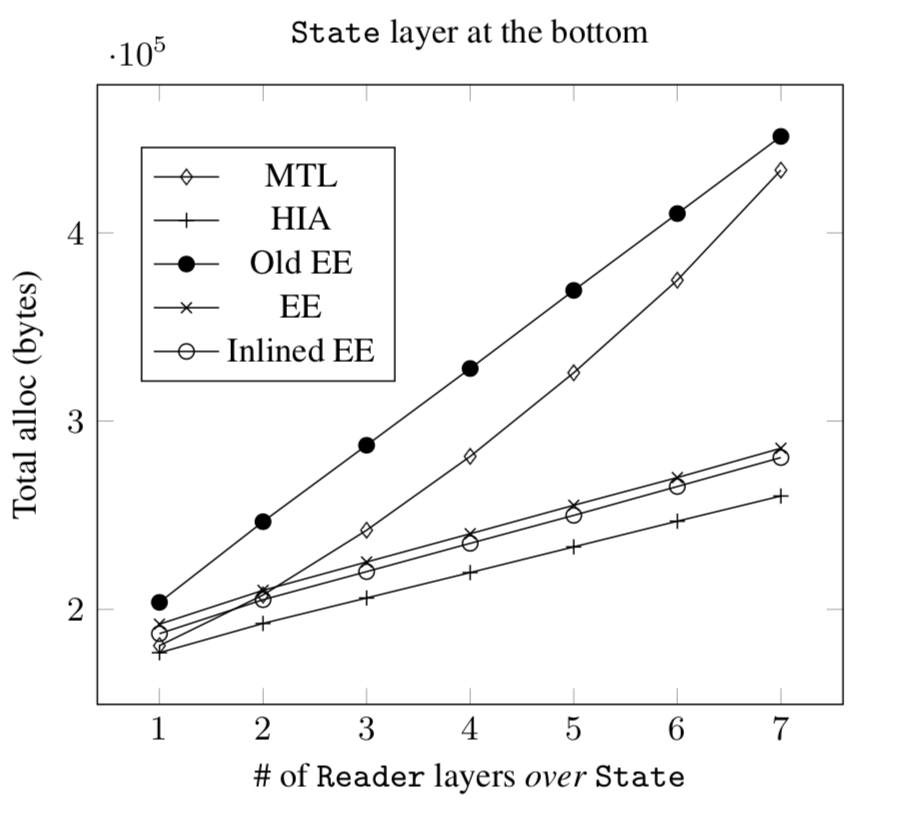
\includegraphics[height=0.7\textheight]{freer-performance.png}
  \cite{freer}
\end{frame}

\section{Similar Systems}

\begin{frame}{Similar Systems}
  \begin{description}
  \item[Handlers in Action] Is is similar to extensible effects, but does not
    group individual effects. \cite{hia}
  \item[Effects] Is a library in idris and additionally allows effects to change
    their types during computation. Enables the use of type level
    computations.~\cite{algebraic-effects-idris}
  \item[PureScript] Is a language with a built-in \texttt{Eff} monad for fine
    grained control over FFI effects.
  \end{description}
\end{frame}

\section{Free structures}

\begin{frame}[fragile]{The Free Monad}
  \begin{lstlisting}
data Free f a
  = Pure a
  | Impure (f (Free f a))

instance Functor f => Monad (Free f a) where
  pure = Pure
  Pure a >>= g = g a
  Impure m >>= g = Impure (fmap (>>= g) m)

iter :: Functor f => (f a -> a) -> Free f a -> a
  \end{lstlisting}
  \begin{itemize}
  \item Treat any \texttt{Functor} like a \texttt{Monad}.
  \item Several combinators are available to quickly create interpreters.
  \item Makes it easy to overload the \texttt{do} notation.
  \end{itemize}
\end{frame}

\begin{frame}[fragile]{Coyoneda}
  \begin{lstlisting}
data Coyoneda f a where
  Coyoneda :: (b -> a) -> f b -> Coyoneda f a

instance Functor (Coyoneda a) where
  fmap f (Coyoneda g v) = Coyoneda (f . g) v

hoistCoyoneda :: (f ~> g) -> Coyoneda f b -> Coyoneda g b

lowerCoyoneda :: Functor f => Coyoneda f a -> f a
  \end{lstlisting}
  \begin{itemize}
  \item Treat any type like a \texttt{Functor}.\note{Used in EE to elide Functor
    constraint on effect data.}
  \item Concrete interpretation can be decided later.
  \end{itemize}
\end{frame}

\section{Conclusion}

\begin{frame}{Lessons Learned}
  \begin{itemize}
  \item Many effects can be expressed in data and handled generically, which
    makes them compose.\note{\texttt{listen} in the writer effect is a prominent
    counter example}
  \item Using generic, transparent data structures rather than stacks removes
    boilerplate and improves performance.
  \item Free structures build complicated structures out of simple, less
    powerful ones.
  \end{itemize}
\end{frame}

\begin{frame}[allowframebreaks]{References}
  \bibliographystyle{alpha}
  \bibliography{bibliography}
\end{frame}
\end{document}